\section{Vectors}

Now we'll move on definining what the first tensor we're seeing is: a vector.

A definition might be, that a vector is a list of numbers, that can be added together and multiplied by a number, but what we're actually describing like this, are the vector components, and not the vector itself.

We have to understand that \textbf{a vector is an invariant}, \textbf{vector components are not}, as they depend on the coordinate systems we use to compute them. \\

Another definition seen frequently is that a vector is like an arrow, having a direction and a magnitude.
You can scale (up or down) vectors multiplying them by scalar numbers, and you can add them by using the tip-to-toe rule.
\textbf{The problem with this definition, is that not all vectors can be visualized as arrows.}
Indeed, the vectors that can be visualized as arrows are a special kind of vectors called "Euclidean vectors" \\

Moving to a different definition, we can say that a vector is a member of a vector space $V$.
A Vector space V is defined as a collection of four things:

\begin{equation}
    \left(V, S, +, \cdot \right)
\end{equation}

\begin{itemize}
    \item $V$ is a set of vectors
    \item $S$ is a set of scalars
    \item $+$ is a sort of addition rule by which we can add vectors together
    \item $\cdot$ is a sort of scaling rule by which we can scale vectors by acting with scalars
\end{itemize}

Now let's say that we have a vector $\vec{v}$ sitting in space and we want to find its components in our basis vectors defined before:
\begin{align*}
    \color{blue} \{\vec{e_1}, \vec{e_2}\} \\
    \color{red}\{\tilde{\vec{e_1}}, \tilde{\vec{e_2}}\}
\end{align*}

This means that we want to measure $\vec{v}$ in two different basis.
Practically, we can do that in the following example, and try to understand how the vector components in different basis relate to each other.

\begin{center}
\input{figures/03-vector-basis-example}
\end{center}

In these basis, we have the forward and backward matrices as follows:

\begin{equation}
    F = 
    \begin{bmatrix}
    2 & -\frac{1}{2}\\
    1 & \frac{1}{4}
    \end{bmatrix}
\end{equation}

\begin{equation}
    B = 
    \begin{bmatrix}
    \frac{1}{4} & \frac{1}{2}\\
    -1 & 2
    \end{bmatrix}
\end{equation}

And if you simply eyeball the diagram and calculate the components of the vector $\color{green}\vec{v}$, you'll find that:

\begin{align*}
    \begingroup\color{blue}\left[ \begin{matrix}
        1 \\
        1.5
    \end{matrix}\right]_{\vec{e_i}}\endgroup & 
    \begingroup\color{red}\left[ \begin{matrix}
        1 \\
        2
    \end{matrix}\right]_{\tilde{\vec{e_i}}}\endgroup
\end{align*}

We saw in the previous section, that, for basis vectors:

\begin{center}
\begin{tikzpicture}[node distance=18mm]
    \node (in) {$\color{blue}\{\vec{e_1}, \vec{e_2}\}$};
    \node[draw, rectangle, minimum width=10mm, minimum height=7mm, right=of in] (F) {$F$};
    \node (out) [right=of F] {$\color{red}\{\tilde{\vec{e_1}}, \tilde{\vec{e_2}}\}$};

    \draw[->] (in) -- (F);
    \draw[->] (F) -- (out);
\end{tikzpicture}

\end{center}

\begin{center}
\begin{tikzpicture}[node distance=18mm]
    \node (in) {$\color{red}\{\tilde{\vec{e_1}}, \tilde{\vec{e_2}}\}$};
    \node[draw, rectangle, minimum width=10mm, minimum height=7mm, right=of in] (B) {$B$};
    \node (out) [right=of B] {$\color{blue}\{\vec{e_1}, \vec{e_2}\}$};

    \draw[->] (in) -- (B);
    \draw[->] (B) -- (out);
\end{tikzpicture}

\end{center}

So let's try and check if following the same logic for the vector components, we can move from one coordinate systems to the other, applying the forward matrix, so:\\

\begin{align*}
    F \begingroup\color{blue}\left[ \begin{matrix}
        1 \\
        1.5
    \end{matrix}\right]_{\vec{e_i}}\endgroup =  
    \begin{bmatrix}
    2 & -\frac{1}{2}\\
    1 & \frac{1}{4}
    \end{bmatrix} \begingroup\color{blue}\left[ \begin{matrix}
        1 \\
        1.5
    \end{matrix}\right]_{\vec{e_i}}\endgroup =
    \begin{bmatrix}
    1.25\\
    1.375
    \end{bmatrix}
\end{align*}

This does not seem right, doens't it? Why don't we try to apply the $B$ matrix instead?

\begin{align*}
    B \begingroup\color{blue}\left[ \begin{matrix}
        1 \\
        1.5
    \end{matrix}\right]_{\vec{e_i}}\endgroup =  
    \begin{bmatrix}
    \frac{1}{4} & \frac{1}{2}\\
    -1 & 2
    \end{bmatrix} \begingroup\color{blue}\left[ \begin{matrix}
        1 \\
        1.5
    \end{matrix}\right]_{\vec{e_i}}\endgroup =
    \begin{bmatrix}
    1\\
    2
    \end{bmatrix}
\end{align*}

\textbf{So this tells us that, for basis vectors, forward matrix brings us from old to new, and backward from new to old, but for vector components, it's the opposite, backward matrix brings us from old to new, and forward from new to old}.
This might seem weird at a first look, but it actually makes sense. Let me give you a couple of examples. Let's start with a simple $\color{green}\vec{v}$ in the basis $\color{blue}\vec{e_i}$ and imagine that you want to describe the same vector (invariant) in a different basis $\color{red}\tilde{\vec{e_i}}$, which is only up-scaled by a factor of 2 wrt to the old basis:

\begin{center}
\begin{minipage}[t]{0.48\linewidth}
\centering
\input{figures/03-vector-scaling-old-basis}
\end{minipage}
\hfill
\begin{minipage}[t]{0.48\linewidth}
\centering
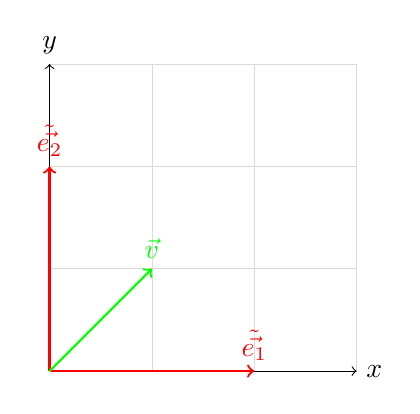
\begin{tikzpicture}[scale=1.3]
  \draw[step=1cm,gray!30,very thin] (0,0) grid (3,3);
  \draw[->] (0,0) -- (3,0) node[right] {$x$};
  \draw[->] (0,0) -- (0,3) node[above] {$y$};
  \draw[->,thick,red] (0,0) -- (2,0) node[above] {$\tilde{\vec{e_1}}$};
  \draw[->,thick,red] (0,0) -- (0,2) node[above] {$\tilde{\vec{e_2}}$};
  \draw[->,thick,green] (0,0) -- (1,1) node[above] {$\vec{v}$};
\end{tikzpicture}

\end{minipage}
\end{center}

If you think about this, as basis vectors scaled up, the vector components have to scale down by the same amount, for the vector itself to be invariant wrt to change of coordinate system. $\color{green}\vec{v}$ "looks" smaller as seen by the new "bigger" coordinate system basis vectors.
Indeed:

\begin{align*}
    \begingroup\color{blue}\left[ \begin{matrix}
        1 \\
        1
    \end{matrix}\right]_{\vec{e_i}}\endgroup & 
    \begingroup\color{red}\left[ \begin{matrix}
        1/2 \\
        1/2
    \end{matrix}\right]_{\tilde{\vec{e_i}}}\endgroup
\end{align*}

The same happens for a simple basis vector rotation:

\begin{center}
\begin{minipage}[t]{0.48\linewidth}
\centering
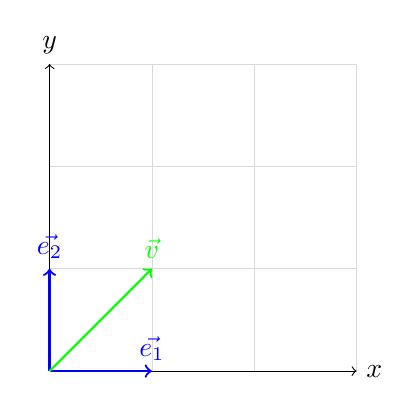
\begin{tikzpicture}[scale=1.3]
  \draw[step=1cm,gray!30,very thin] (0,0) grid (3,3);
  \draw[->] (0,0) -- (3,0) node[right] {$x$};
  \draw[->] (0,0) -- (0,3) node[above] {$y$};
  \draw[->,thick,blue] (0,0) -- (1,0) node[above] {$\vec{e_1}$};
  \draw[->,thick,blue] (0,0) -- (0,1) node[above] {$\vec{e_2}$};
  \draw[->,thick,green] (0,0) -- (1,1) node[above] {$\vec{v}$};
\end{tikzpicture}

\end{minipage}
\hfill
\begin{minipage}[t]{0.48\linewidth}
\centering
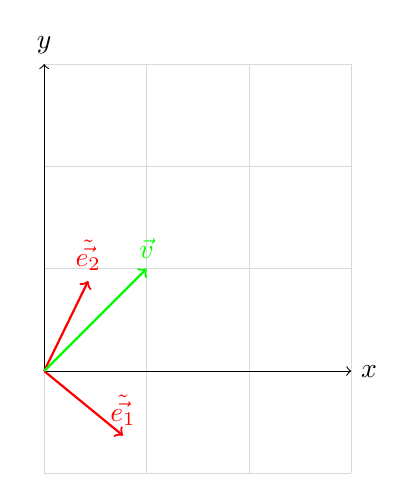
\begin{tikzpicture}[scale=1.3]
  \draw[step=1cm,gray!30,very thin] (0,-1) grid (3,3);
  \draw[->] (0,0) -- (3,0) node[right] {$x$};
  \draw[->] (0,0) -- (0,3) node[above] {$y$};
  \draw[->,thick,red] (0,0) -- (0.77,-0.63) node[above] {$\tilde{\vec{e_1}}$};
  \draw[->,thick,red] (0,0) -- (0.43,0.88) node[above] {$\tilde{\vec{e_2}}$};
  \draw[->,thick,green] (0,0) -- (1,1) node[above] {$\vec{v}$};
\end{tikzpicture}

\end{minipage}
\end{center}

In this case, intuitively and from the picture, it's clearly visible that a clockwise rotation of the basis vectors corresponds to a counter-clockwise rotation of the vector components. \\

Next step would be proving this in more dimentions. We can write the vector as a linear combination of its vector components in two different coordinate systems / basis vectors:

\begin{align*}
    \begingroup\color{green}\vec{v}\endgroup &= \begingroup\color{cyan}v_1\endgroup\begingroup\color{blue}\vec{e_1}\endgroup + \begingroup\color{cyan}v_2\endgroup\begingroup\color{blue}\vec{e_2}\endgroup + \cdots + \begingroup\color{cyan}v_n\endgroup\begingroup\color{blue}\vec{e_n}\endgroup = \sum_{j=1}^{n} \begingroup\color{cyan}v_j\endgroup \begingroup\color{blue}\vec{e_j}\endgroup \\
    \begingroup\color{green}\vec{v}\endgroup &= \begingroup\color{magenta}\tilde{v_1}\endgroup\begingroup\color{red}\tilde{\vec{e_1}}\endgroup + \begingroup\color{magenta}\tilde{v_2}\endgroup\begingroup\color{red}\tilde{\vec{e_2}}\endgroup + \cdots + \begingroup\color{magenta}\tilde{v_n}\endgroup\begingroup\color{red}\tilde{\vec{e_n}}\endgroup = \sum_{j=1}^{n} \begingroup\color{magenta}\tilde{v_j}\endgroup \begingroup\color{red}\tilde{\vec{e_j}}\endgroup
\end{align*}

Bringing back our basis vector forward and backward transformations:

\begin{subequations}
\begin{empheq}[box=\widefbox]{align}
    \begingroup\color{red}\tilde{\vec{e_i}}\endgroup = \sum_{j=1}^{n} F_{ji} \begingroup\color{blue}\vec{e_j}\endgroup \\
    \begingroup\color{blue}\vec{e_i}\endgroup = \sum_{j=1}^{n} B_{ji} \begingroup\color{red}\tilde{\vec{e_j}}\endgroup
\end{empheq}
\end{subequations}

We can write:

\begin{align*}
    \begingroup\color{green}\vec{v}\endgroup &= \sum_{j=1}^{n} \begingroup\color{cyan}v_j\endgroup \begingroup\color{blue}\vec{e_j}\endgroup = \sum_{j=1}^{n} \begingroup\color{cyan}v_j\endgroup \left(\sum_{i=1}^{n} B_{ij} \begingroup\color{red}\tilde{\vec{e_i}}\endgroup\right) = \sum_{i=1}^{n}\left(\sum_{j=1}^{n}B_{ij}\begingroup\color{cyan}v_j\endgroup\right)\begingroup\color{red}\tilde{\vec{e_i}}\endgroup
\end{align*}

As you can see, \textbf{this actually proves that, to move from the old components to the new components, we use the backward transformation matrix}, and \textbf{to move from the new components to the old components, we use the forward transformation matrix}:

\begin{subequations}
\begin{empheq}[box=\widefbox]{align}
    \begingroup\color{magenta}\tilde{v_i}\endgroup = \sum_{j=1}^{n} B_{ij} \begingroup\color{cyan}v_j\endgroup \\
    \begingroup\color{cyan}v_i\endgroup = \sum_{j=1}^{n} F_{ij} \begingroup\color{magenta}\tilde{v_j}\endgroup
\end{empheq}
\end{subequations}

So, summarizing what we've learned so far, we know the transformation rules that basis vectors and vector components obey:

\begin{center}
\begin{minipage}[t]{0.48\linewidth}
\centering
\begin{subequations}
\begin{empheq}[box=\widefbox]{align}
    \begingroup\color{red}\tilde{\vec{e_i}}\endgroup = \sum_{j=1}^{n} F_{ji} \begingroup\color{blue}\vec{e_j}\endgroup \\
    \begingroup\color{blue}\vec{e_i}\endgroup = \sum_{j=1}^{n} B_{ji} \begingroup\color{red}\tilde{\vec{e_j}}\endgroup
\end{empheq}
\end{subequations}
\end{minipage}
\hfill
\begin{minipage}[t]{0.48\linewidth}
\centering
\begin{subequations}
\begin{empheq}[box=\widefbox]{align}
    \begingroup\color{magenta}\tilde{v_i}\endgroup = \sum_{j=1}^{n} B_{ij} \begingroup\color{cyan}v_j\endgroup \\
    \begingroup\color{cyan}v_i\endgroup = \sum_{j=1}^{n} F_{ij} \begingroup\color{magenta}\tilde{v_j}\endgroup
\end{empheq}
\end{subequations}
\end{minipage}
\end{center}

Since the vector components behave contrary to the basis vectors, we say that they are contra-variant. \\
We'll see later indeed, that vectors are contra-variant tensors and from now on, we're going to make a small change in the way we write vector components due to this behavior, and we're writing them with the index on top and not on the bottom:

\begin{align*}
    \begingroup\color{green}\vec{v}\endgroup = \sum_{i=1}^{n} \begingroup\color{cyan}v^i\endgroup \begingroup\color{blue}\vec{e_i}\endgroup = \sum_{i=1}^{n} \begingroup\color{magenta}\tilde{v^i}\endgroup \begingroup\color{red}\tilde{\vec{e_i}}\endgroup
\end{align*}
